\documentclass[12pt,letterpaper]{article}
\usepackage{graphicx,textcomp}
\usepackage{natbib}
\usepackage{setspace}
\usepackage{fullpage}
\usepackage{color}
\usepackage[reqno]{amsmath}
\usepackage{amsthm}
\usepackage{fancyvrb}
\usepackage{amssymb,enumerate}
\usepackage[all]{xy}
\usepackage{endnotes}
\usepackage{lscape}
\newtheorem{com}{Comment}
\usepackage{float}
\usepackage{hyperref}
\newtheorem{lem} {Lemma}
\newtheorem{prop}{Proposition}
\newtheorem{thm}{Theorem}
\newtheorem{defn}{Definition}
\newtheorem{cor}{Corollary}
\newtheorem{obs}{Observation}
\usepackage[compact]{titlesec}
\usepackage{dcolumn}
\usepackage{tikz}
\usetikzlibrary{arrows}
\usepackage{multirow}
\usepackage{xcolor}
\newcolumntype{.}{D{.}{.}{-1}}
\newcolumntype{d}[1]{D{.}{.}{#1}}
\definecolor{light-gray}{gray}{0.65}
\usepackage{url}
\usepackage{listings}
\usepackage{color}

\definecolor{codegreen}{rgb}{0,0.6,0}
\definecolor{codegray}{rgb}{0.5,0.5,0.5}
\definecolor{codepurple}{rgb}{0.58,0,0.82}
\definecolor{backcolour}{rgb}{0.95,0.95,0.92}

\lstdefinestyle{mystyle}{
	backgroundcolor=\color{backcolour},   
	commentstyle=\color{codegreen},
	keywordstyle=\color{magenta},
	numberstyle=\tiny\color{codegray},
	stringstyle=\color{codepurple},
	basicstyle=\footnotesize,
	breakatwhitespace=false,         
	breaklines=true,                 
	captionpos=b,                    
	keepspaces=true,                 
	numbers=left,                    
	numbersep=5pt,                  
	showspaces=false,                
	showstringspaces=false,
	showtabs=false,                  
	tabsize=2
}
\lstset{style=mystyle}
\newcommand{\Sref}[1]{Section~\ref{#1}}
\newtheorem{hyp}{Hypothesis}

\title{Problem Set 3}
\date{Due: November 11, 2024}
\author{Applied Stats/Quant Methods 1
	\\ Jianxiong Wu---23354731}

\begin{document}
	\maketitle
	\section*{Instructions}
	\begin{itemize}
		\item Please show your work! You may lose points by simply writing in the answer. If the problem requires you to execute commands in \texttt{R}, please include the code you used to get your answers. Please also include the \texttt{.R} file that contains your code. If you are not sure if work needs to be shown for a particular problem, please ask.
	\item Your homework should be submitted electronically on GitHub.
	\item This problem set is due before 23:59 on Sunday November 11, 2024. No late assignments will be accepted.

	\end{itemize}

		\vspace{.25cm}
	
\noindent In this problem set, you will run several regressions and create an add variable plot (see the lecture slides) in \texttt{R} using the \texttt{incumbents\_subset.csv} dataset. Include all of your code.

	\vspace{.5cm}
\section*{Question 1}
\vspace{.25cm}
\noindent We are interested in knowing how the difference in campaign spending between incumbent and challenger affects the incumbent's vote share. 
	\begin{enumerate}
		\item Run a regression where the outcome variable is \texttt{voteshare} and the explanatory variable is \texttt{difflog}.	
		
		\lstinputlisting[language=R, firstline=37, lastline=39]{PS03_Jianxiong Wu_23354731.R}  
		
		\begin{verbatim} 
		Results: 
		Call:
		lm(formula = voteshare ~ difflog, data = inc.sub)
		
		Residuals:
		Min       1Q   Median       3Q      Max 
		-0.26832 -0.05345 -0.00377  0.04780  0.32749 
		
		Coefficients:
		Estimate Std. Error t value Pr(>|t|)    
		(Intercept) 0.579031   0.002251  257.19   <2e-16 ***
		difflog     0.041666   0.000968   43.04   <2e-16 ***
		---
		Signif. codes:  0 ‘***’ 0.001 ‘**’ 0.01 ‘*’ 0.05 ‘.’ 0.1 ‘ ’ 1
		
		Residual standard error: 0.07867 on 3191 degrees of freedom
		Multiple R-squared:  0.3673,	Adjusted R-squared:  0.3671 
		F-statistic:  1853 on 1 and 3191 DF,  p-value: < 2.2e-16
		
		
		This regression shows that the difference in campaign spending 
		between incumbent and challenger has a significant positive effect 
		on the incumbent's vote share. On average, each unit increase in 
		difflog increases the incumbent's vote share by about 0.042.
		\end{verbatim}	
		
		\item Make a scatterplot of the two variables and add the regression line. 	
		
		\lstinputlisting[language=R, firstline=41, lastline=48]{PS03_Jianxiong Wu_23354731.R}  
		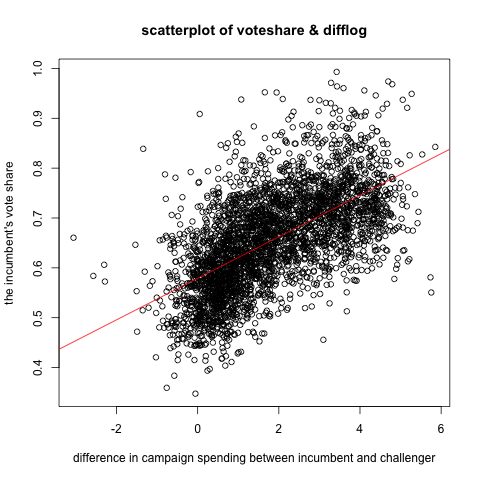
\includegraphics[width=.75\textwidth]{q1_regression.png}
		
		\item Save the residuals of the model in a separate object.
		
		\lstinputlisting[language=R, firstline=50, lastline=52]{PS03_Jianxiong Wu_23354731.R}  
		
		\item Write the prediction equation.
		
		\begin{verbatim} 
		Results: 
		voteshare = intercept + coefficient * difflog
		voteshare = 0.579031 + 0.041666 * difflog
		\end{verbatim}
		
	\end{enumerate}
	
\newpage

\section*{Question 2}
\noindent We are interested in knowing how the difference between incumbent and challenger's spending and the vote share of the presidential candidate of the incumbent's party are related.	\vspace{.25cm}
	\begin{enumerate}
		\item Run a regression where the outcome variable is \texttt{presvote} and the explanatory variable is \texttt{difflog}.
		
		\lstinputlisting[language=R, firstline=61, lastline=63]{PS03_Jianxiong Wu_23354731.R}  
		
		\begin{verbatim}
		Results: 
		Call:
		lm(formula = presvote ~ difflog, data = inc.sub)
		
		Residuals:
		Min       1Q   Median       3Q      Max 
		-0.32196 -0.07407 -0.00102  0.07151  0.42743 
		
		Coefficients:
		Estimate Std. Error t value Pr(>|t|)    
		(Intercept) 0.507583   0.003161  160.60   <2e-16 ***
		difflog     0.023837   0.001359   17.54   <2e-16 ***
		---
		Signif. codes:  0 ‘***’ 0.001 ‘**’ 0.01 ‘*’ 0.05 ‘.’ 0.1 ‘ ’ 1
		
		Residual standard error: 0.1104 on 3191 degrees of freedom
		Multiple R-squared:  0.08795,	Adjusted R-squared:  0.08767 
		F-statistic: 307.7 on 1 and 3191 DF,  p-value: < 2.2e-16
		
		
		This regression shows that the difference in campaign spending 
		between incumbent and challenger has a significant positive effect 
		on the vote share of the presidential candidate. On average, each 
		unit increase in difflog increases the vote share of the presidential 
		candidate by about 0.024.
		\end{verbatim}
		
		\item Make a scatterplot of the two variables and add the regression line. 
		
		\lstinputlisting[language=R, firstline=65, lastline=72]{PS03_Jianxiong Wu_23354731.R}  
		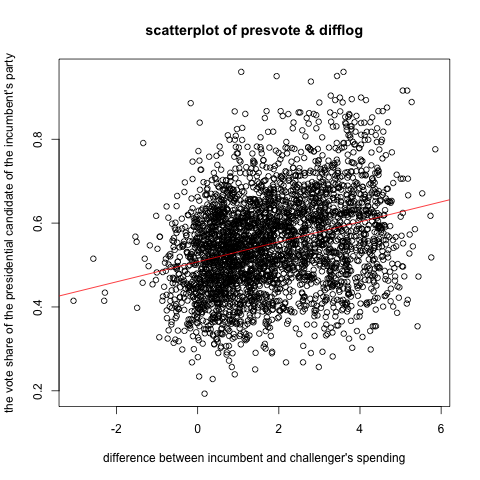
\includegraphics[width=.75\textwidth]{q2_regression.png}
		
		\item Save the residuals of the model in a separate object.
		
		\lstinputlisting[language=R, firstline=74, lastline=76]{PS03_Jianxiong Wu_23354731.R}  
		
		\item Write the prediction equation.
		
		\begin{verbatim} 
		Results: 
		presvote = intercept + coefficient * difflog
		presvote = 0.507583 + 0.023837 * difflog
		\end{verbatim}
		
	\end{enumerate}
	
	\newpage	
\section*{Question 3}

\noindent We are interested in knowing how the vote share of the presidential candidate of the incumbent's party is associated with the incumbent's electoral success.
	\vspace{.25cm}
	\begin{enumerate}
		\item Run a regression where the outcome variable is \texttt{voteshare} and the explanatory variable is \texttt{presvote}.
		
		\lstinputlisting[language=R, firstline=85, lastline=87]{PS03_Jianxiong Wu_23354731.R} 
		
		\begin{verbatim} 
		Results: 
		Call:
		lm(formula = voteshare ~ presvote, data = inc.sub)
		
		Residuals:
		Min       1Q   Median       3Q      Max 
		-0.27330 -0.05888  0.00394  0.06148  0.41365 
		
		Coefficients:
		Estimate Std. Error t value Pr(>|t|)    
		(Intercept) 0.441330   0.007599   58.08   <2e-16 ***
		presvote    0.388018   0.013493   28.76   <2e-16 ***
		---
		Signif. codes:  0 ‘***’ 0.001 ‘**’ 0.01 ‘*’ 0.05 ‘.’ 0.1 ‘ ’ 1
		
		Residual standard error: 0.08815 on 3191 degrees of freedom
		Multiple R-squared:  0.2058,	Adjusted R-squared:  0.2056 
		F-statistic:   827 on 1 and 3191 DF,  p-value: < 2.2e-16
		
		
		This regression shows that the vote share of the presidential 
		candidate has a significant positive effect on the incumbent’s 
		vote share. On average, each unit increase in prevote increases 
		the incumbent’s vote share by about 0.388.
		\end{verbatim}
		
		
		\item Make a scatterplot of the two variables and add the regression line. 
		
		\lstinputlisting[language=R, firstline=89, lastline=96]{PS03_Jianxiong Wu_23354731.R}  
		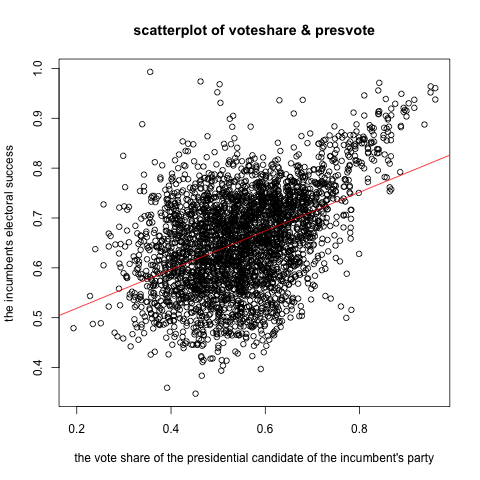
\includegraphics[width=.75\textwidth]{q3_regression.png}
		
		\item Write the prediction equation.
		
		\begin{verbatim} 
		Results: 
		voteshare = intercept + coefficient * presvote
		voteshare = 0.441330 + 0.388018 * presvote
		\end{verbatim}
		
	\end{enumerate}
	

\newpage	
\section*{Question 4}
\noindent The residuals from part (a) tell us how much of the variation in \texttt{voteshare} is $not$ explained by the difference in spending between incumbent and challenger. The residuals in part (b) tell us how much of the variation in \texttt{presvote} is $not$ explained by the difference in spending between incumbent and challenger in the district.
	\begin{enumerate}
		\item Run a regression where the outcome variable is the residuals from Question 1 and the explanatory variable is the residuals from Question 2.
		
		\lstinputlisting[language=R, firstline=105, lastline=107]{PS03_Jianxiong Wu_23354731.R} 
		
		\begin{verbatim} 
		Call:
		lm(formula = q1_residuals ~ q2_residuals, data = inc.sub)
		
		Residuals:
		Min       1Q   Median       3Q      Max 
		-0.25928 -0.04737 -0.00121  0.04618  0.33126 
		
		Coefficients:
		Estimate Std. Error t value Pr(>|t|)    
		(Intercept)  -1.942e-18  1.299e-03    0.00        1    
		q2_residuals  2.569e-01  1.176e-02   21.84   <2e-16 ***
		---
		Signif. codes:  0 ‘***’ 0.001 ‘**’ 0.01 ‘*’ 0.05 ‘.’ 0.1 ‘ ’ 1
		
		Residual standard error: 0.07338 on 3191 degrees of freedom
		Multiple R-squared:   0.13,	Adjusted R-squared:  0.1298 
		F-statistic:   477 on 1 and 3191 DF,  p-value: < 2.2e-16
		
		
		This regression shows that question2 residuals has a significant 
		positive effect on question1 residuals. On average, each unit 
		increase in question2 residuals increases question1 residuals by 
		about 0.2569.
		\end{verbatim}
		
		\item Make a scatterplot of the two residuals and add the regression line. 
		
		\lstinputlisting[language=R, firstline=109, lastline=116]{PS03_Jianxiong Wu_23354731.R}  
		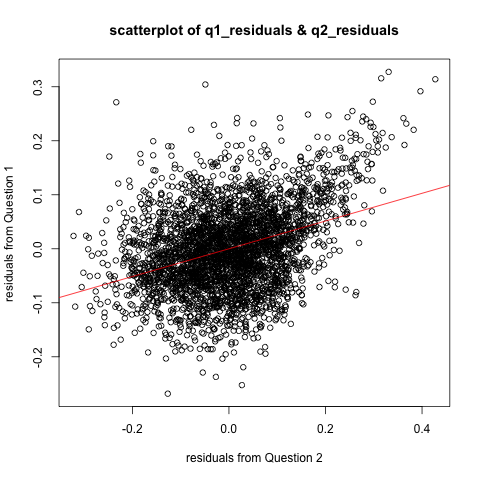
\includegraphics[width=.75\textwidth]{q4_regression.png}
		
		\item Write the prediction equation.
		
		\begin{verbatim} 
		Results: 
		q1_residuals = intercept + coefficient * q2_residuals
		q1_residuals = (-1.942e-18) + (2.569e-01) * q2_residuals
		\end{verbatim}
		
	\end{enumerate}
	
	\newpage	

\section*{Question 5}
\noindent What if the incumbent's vote share is affected by both the president's popularity and the difference in spending between incumbent and challenger? 
	\begin{enumerate}
		\item Run a regression where the outcome variable is the incumbent's \texttt{voteshare} and the explanatory variables are \texttt{difflog} and \texttt{presvote}.
		
		\lstinputlisting[language=R, firstline=125, lastline=127]{PS03_Jianxiong Wu_23354731.R} 
		
		\begin{verbatim} 
		Results: 
		Call:
		lm(formula = voteshare ~ difflog + presvote, data = inc.sub)
		
		Residuals:
		Min       1Q   Median       3Q      Max 
		-0.25928 -0.04737 -0.00121  0.04618  0.33126 
		
		Coefficients:
		Estimate Std. Error t value Pr(>|t|)    
		(Intercept) 0.4486442  0.0063297   70.88   <2e-16 ***
		difflog     0.0355431  0.0009455   37.59   <2e-16 ***
		presvote    0.2568770  0.0117637   21.84   <2e-16 ***
		---
		Signif. codes:  0 ‘***’ 0.001 ‘**’ 0.01 ‘*’ 0.05 ‘.’ 0.1 ‘ ’ 1
		
		Residual standard error: 0.07339 on 3190 degrees of freedom
		Multiple R-squared:  0.4496,	Adjusted R-squared:  0.4493 
		F-statistic:  1303 on 2 and 3190 DF,  p-value: < 2.2e-16
		
		
		This regression is a multivariate regression, with both difflog 
		and prevote as independent variables. On average, when difflog 
		is held constant, each unit increase in prevote increases the 
		incumbent's vote share by approximately 0.2569. When prevote 
		is held constant, each unit increase in difflog increases the 
		incumbent's vote share increases by approximately 0.0355. 
		Both explanatory variables have a significant positive effect on 
		the incumbent's vote share.
		\end{verbatim}
\newpage	
		\item Write the prediction equation.
		
		\begin{verbatim} 
		Results: 
		voteshare = intercept + coefficient1 * difflog + coefficient2 * presvote
		voteshare = 0.448644 + 0.035543 * difflog + 0.256887 * presvote
		\end{verbatim}
		
		\item What is it in this output that is identical to the output in Question 4? Why do you think this is the case?
		
		\begin{verbatim} 
		Results: 
		The coefficient of presvote in the q5_regression in Question 5 is the 
		same as the coefficient of q2_residuals in the q4_regression in 
		Question 4, which is 0.2569. The reason for this is that in the 
		q5_regression, difflog is used as an explanatory variable along with 
		presvote. And in q4_regression, the residuals of voteshare ~ difflog 
		and presvote ~ difflog are used for the regression. So there is an 
		independent effect of presvote on vote share after controlling for 
		difflog.
		\end{verbatim}
		
	\end{enumerate}




\end{document}
